\documentclass{article}
%babel
\usepackage[romanian]{babel}
%
\usepackage{graphicx}%dorim să importăm grafică
%\renewcommand{\tablename}{Tabelul}
%titlu
\title{Legile lui Newton}
\author{Pleanta Mihai-Alexandru}
\begin{document}
\maketitle	
\begin{abstract}
Rezumat: In lucrare sunt prezentate elemente introductive privind legile lui Newton
\end{abstract}
\section{Introducere}
Legile lui Newton (sau principiile fundamentale ale mecanicii) sunt trei legi ale fizicii care dau o relație directă între forțele care acționează asupra unui corp și mișcarea acelui corp. Ele au fost enunțate de Sir Isaac Newton (bazat și pe studiile lui Galilei) în lucrarea sa Philosophiae Naturalis Principia Mathematica (1687). Aceste legi formează baza mecanicii clasice.
\section{Principiul I și al II-lea al mecanicii}
Fragment cu \verb+tabbing+:
\begin{tabbing}
s=0\\
fo\= r i=0:n\\
\> s=s+1;\\\=
end\\
s
\end{tabbing}
Tabel cu \verb+table+ și \verb+tabular+:
\begin{table}[htpb]
\centering
\begin{tabular}{llc}
\multicolumn{3}{c}{Prima linie extinsă}\\\hline
Nr.&Element&Simbol\\\hline
1.&rezistență&$R$\\
2.&inductivitate&$L$\\
3.&capacitate&$C$

\end{tabular}
\caption{Primul meu tabel}\label{tab:RLC}
\end{table}
Conform simbolurile din tabela \ref{tab:RLC},...
\section{Inserare de grafică}
Aici se afisează graficul funcției sinus.
\begin{figure}[ht]
\centering
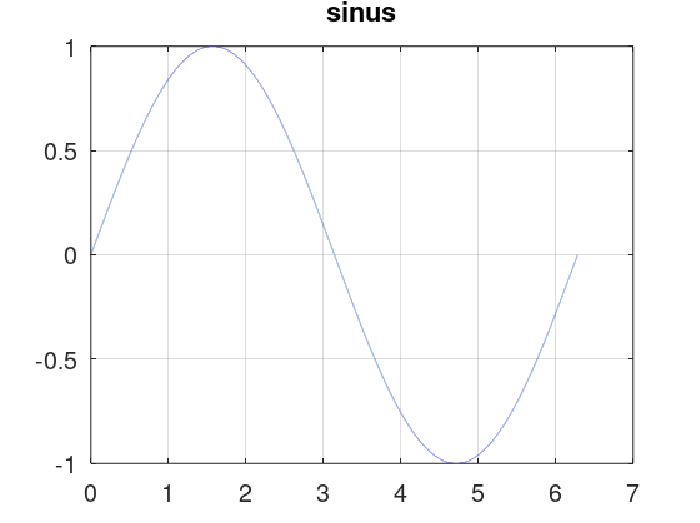
\includegraphics[scale=0.9]{SINUS.pdf}
\caption{Sinus}. \label{fig:sin}
\end{figure}
\end{document}